\documentclass{article}

\usepackage[margin=1.0in]{geometry}
\usepackage{graphicx}
\usepackage{amsmath}
\usepackage{float}
\usepackage{enumitem}
\usepackage{gensymb}

\title{CSC 577 HW7}
\date{3/20/2019}
\author{Simon Swenson}

\begin{document}

\pagenumbering{gobble}
\maketitle
\pagenumbering{arabic}

\section{Introduction}

\begin{figure}[!ht]
	\centering
	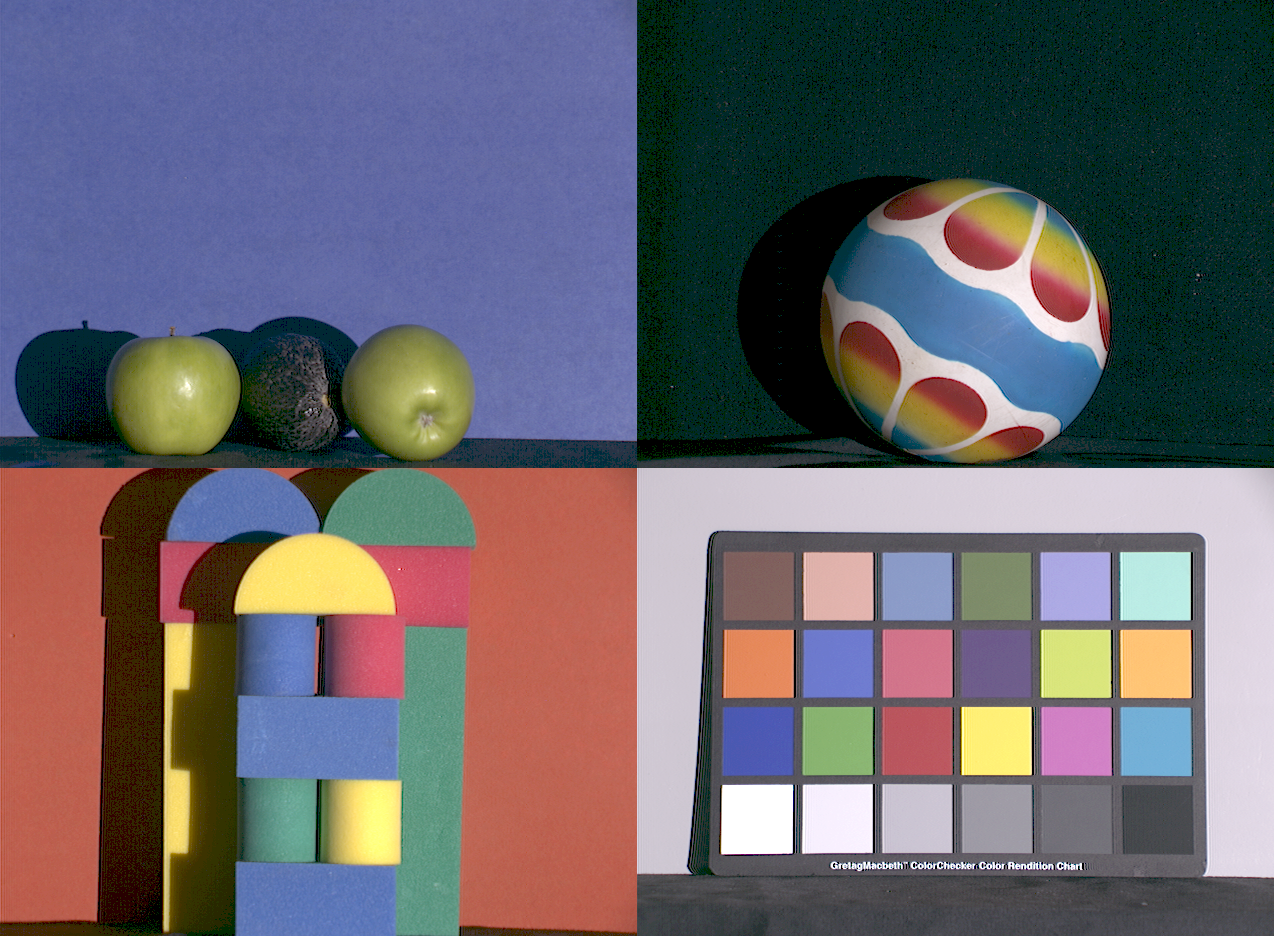
\includegraphics[width=120mm]{figs/four-scenes_cc.png}
	\caption{The four scenes explored in this assignment, lit by a white light, 
        gamma corrected, and exposure increased.}
\end{figure}

In this assignment, we were presented various scenes lit by two different 
lights: a deep blue light and a pure white light. We explored various ways to 
estimate the red, green, and 
blue values for these lights, including using white patches, using the 
"max RGB" approach, using the "gray world" approach, and minimizing the mean 
squared error, and using a built-in MATLAB solver to find the minimum solution 
to RMSE r,g. Each of these methods has advantages and disadvantages, which we 
saw on visual inspection, by calculating the angular error, and by calculating 
the RMSE r,g.

\section{Estimating Light Values from White Patches}

Similar to how we used a regular grid over $R^3$ to calibrate a camera, we can 
use a plain white patch to find the red, green, and blue values for a light. 
This is essentially an "oracle" approach, since we manually select the pixels 
which are within the white patch and know that that patch is pure white. This 
yields the following two colors for the lights:

\begin{tabular}{r | r r r}
                              & Red & Green & Blue \\
    \hline                                         \\
    syl-50MR16Q (white light) & 239 &   222 &  250 \\
      solux-4100 (blue light) & 131 &   159 &  250
\end{tabular}

The angular error between these two light colors is 0.2416.
From 
there, we use the diagonal color model to transform each pixel in the source 
image, using the following equation for the diagonal color model:

$$
\begin{bmatrix}
R_2 \\
G_2 \\
B_2
\end{bmatrix} = \begin{bmatrix}
\frac{R_{L2}}{R_{L1}} &                       &                       \\
                      & \frac{G_{L2}}{G_{L1}} &                       \\
                      &                       & \frac{B_{L2}}{B_{L1}}
\end{bmatrix} \begin{bmatrix}
R_1 \\
G_1 \\
B_1
\end{bmatrix}
$$

Using 
this approach yields good results, but the corrected image appears slightly 
darker than the target image. However, upon closer inspection, the white patch 
has the correct average color. The RMSE r,g results between the original two 
images and the predicted image and the target image are shown below. The 
prediction image decreases the RMSE r,g by more than half:

\begin{tabular}{r | r}
    blue-to-white RMSE r,g & 0.0746 \\
    predicted-to-white RMSE r,g & 0.0335
\end{tabular}

However, qualitatively, even though the RMSE r,g was only reduced by a little 
more than half, the image looks \textit{much} closer to the target image.

\begin{figure}[!ht]
	\centering
	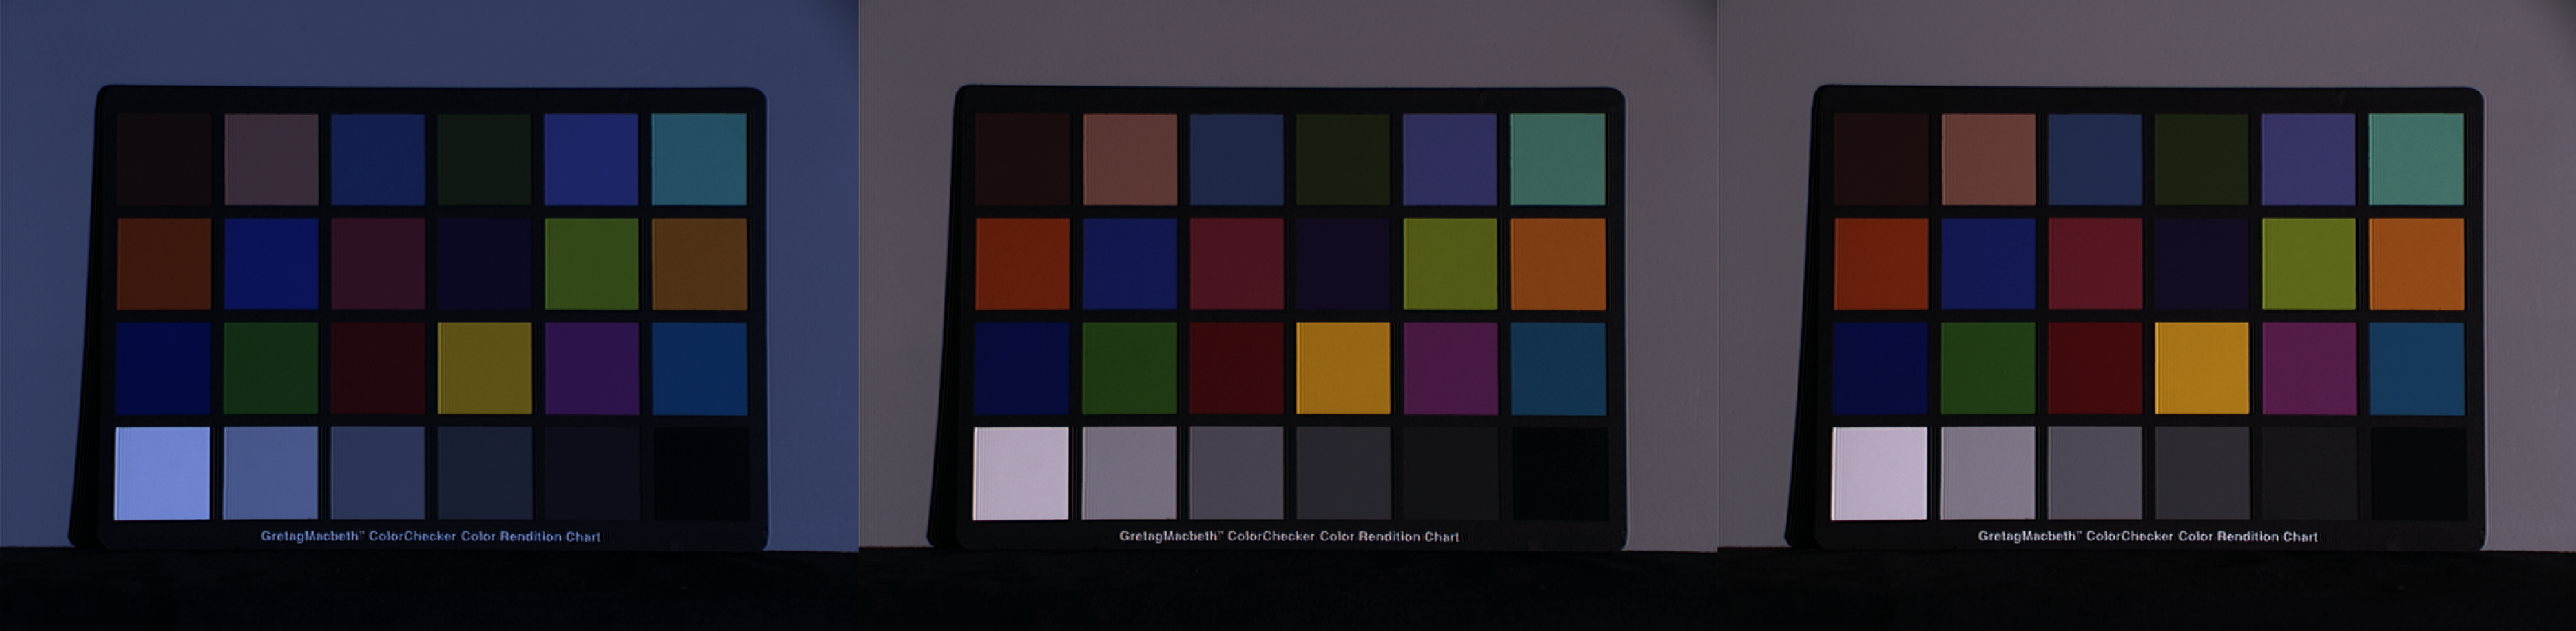
\includegraphics[width=160mm]{figs/macbeth-comparison.png}
	\caption{Left: A color swatch lit by the blue light. This is the source. 
        Center: The color 
        swatch transformed from the blue light space to the white light space 
        using the diagonal color model. 
        This is the prediction.
        Right: A color swatch lit by the white light. This is the target.}
\end{figure}

What could be the reason for the white patch being correct, but the rest of the 
scene appearing darker? One possible explanation is that the patch is not pure 
white. Any impurity of the color could cause the transformation to fail, since 
it will not give an accurate reading for the light values.

\section{Estimating Light Values using Max RGB}

Now that we have a good baseline for how well we could calculate the light 
values in an oracle situation, we can compare two different approaches to that 
one and see how well we can do without perfect information. The first approach 
is called "max RGB." The algorithm finds the maximum value in each of the three 
channels of the image and uses that as the value for the light:

$$
\begin{bmatrix}
    R^U_W \\
    G^U_W \\
    B^U_W
\end{bmatrix} = \begin{bmatrix}
    max_{pix} R \\
    max_{pix} G \\
    max_{pix} B
\end{bmatrix}
$$

Intuitively, this approach should fair well when the image contains dielectric 
materials, since such materials have specular highlights, which should match the 
color of the light closely. This should also work well when there is any sort of 
white patch in the image, since that will dominate the "max" values. We explore 
this approach using three different scenes, a scene with 
several apples and a blue background, a scene with a ball and a black background, 
and a scene with blocks and a red background. Doing so leads to the following 
predicted lights:

\begin{tabular}{r | r r r}
                 & Red & Green & Blue \\
    \hline                            \\
    Apples Light & 182 &   228 &  250 \\
      Ball Light & 112 &   143 &  250 \\
    Blocks Light & 250 &   242 &  209
\end{tabular}

and the quantitative results:

\begin{tabular}{r | r r}
                 & Angular Error & RMSE r,g Error \\
    \hline                                        \\
    Apples Light &        0.1713 &         0.0431 \\
      Ball Light &        0.0637 &         0.0661 \\
    Blocks Light &        0.3484 &         0.0746
\end{tabular}

And the qualitative results:

\begin{figure}[!ht]
	\centering
	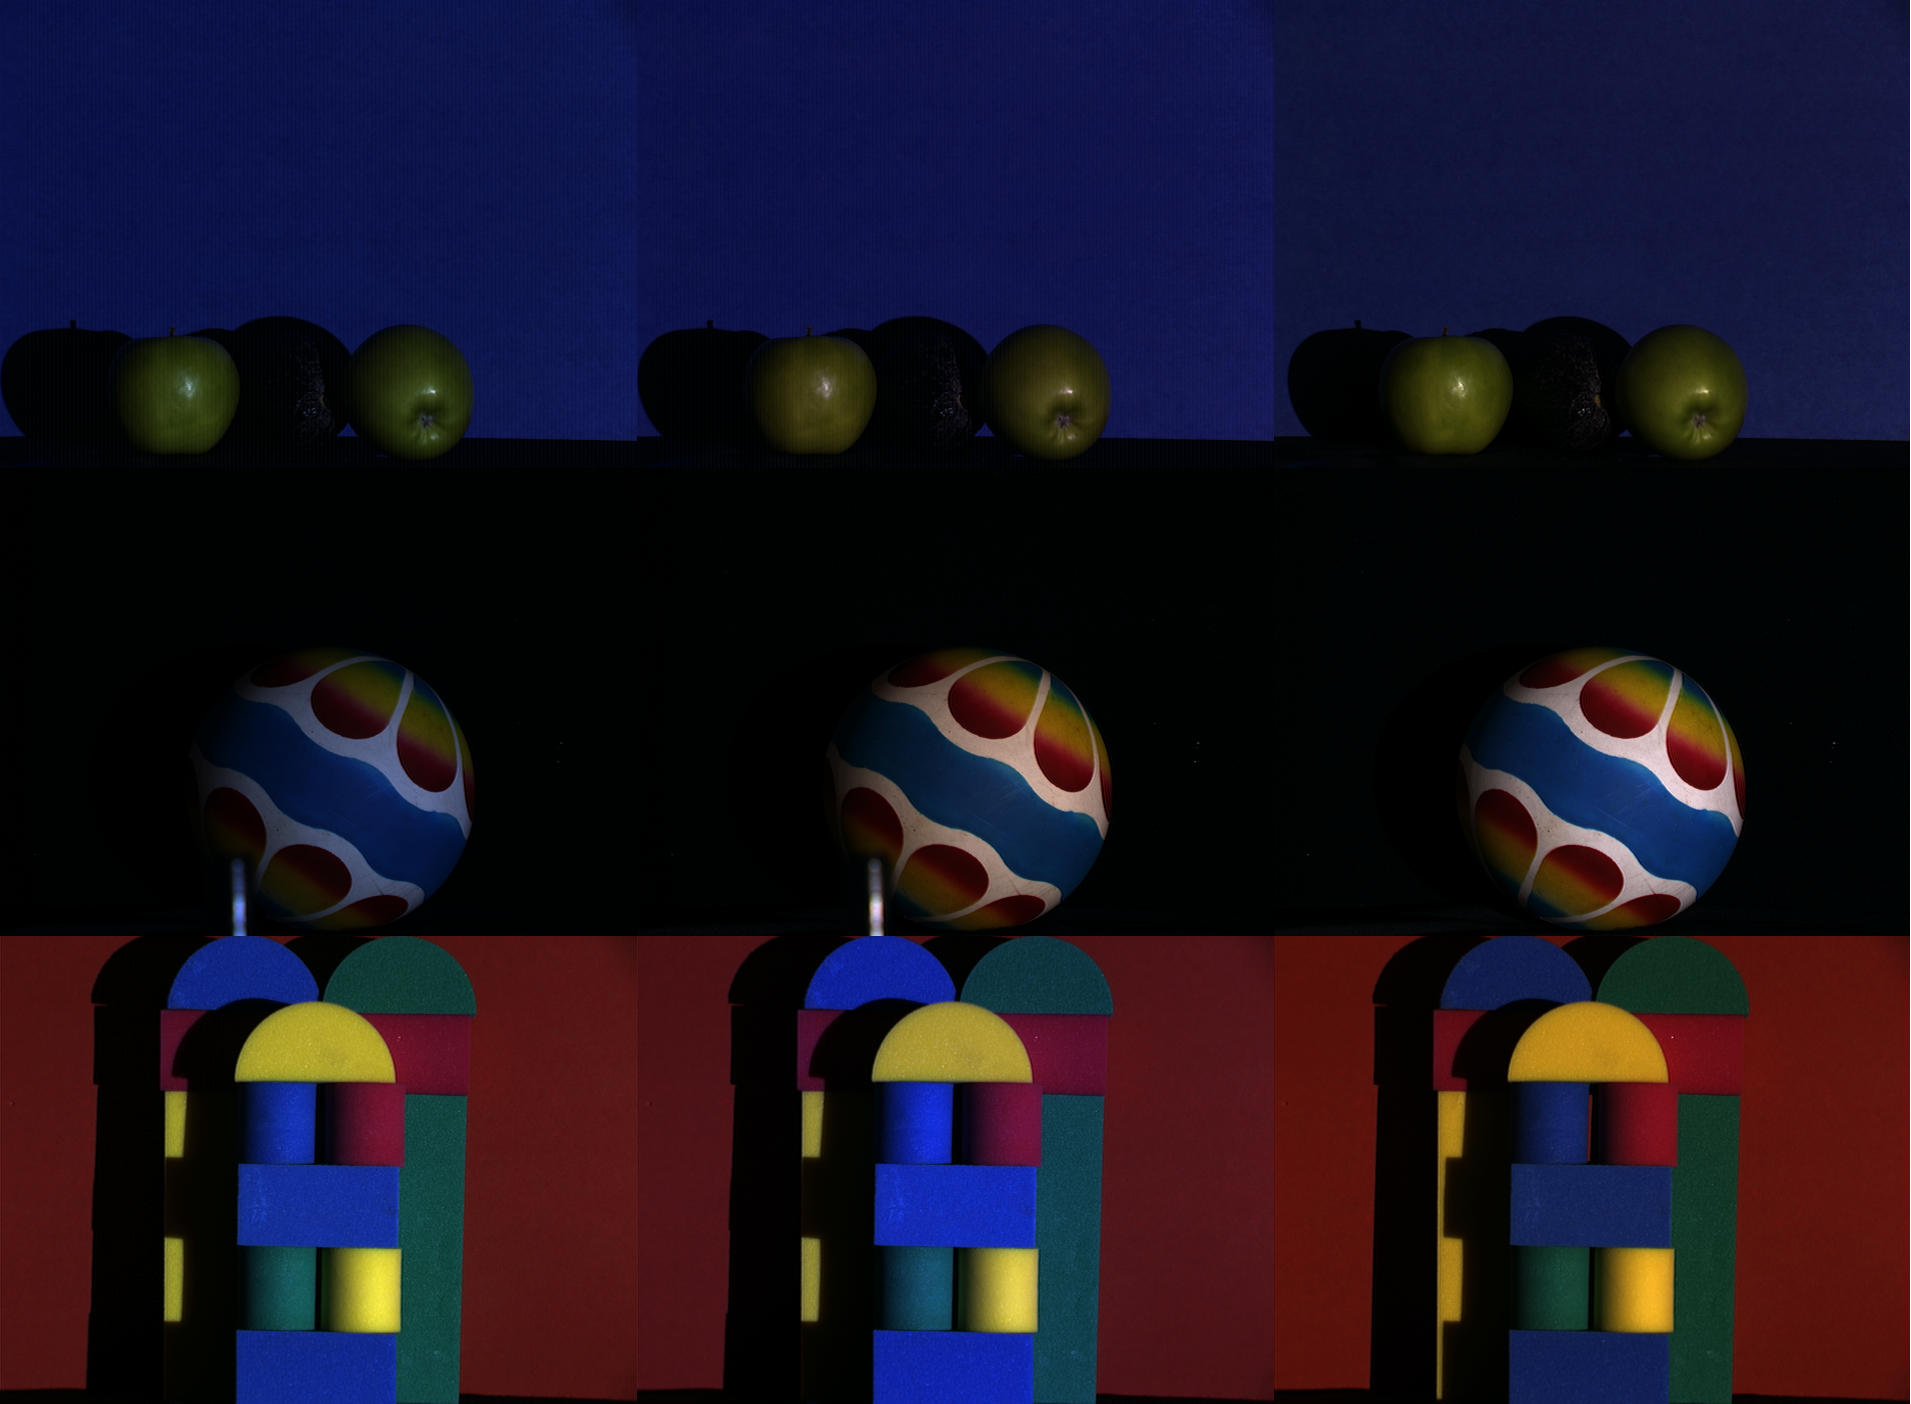
\includegraphics[width=120mm]{figs/results-maxrgb-3x3.png}
	\caption{Left: The three scenes (apples, ball, blocks) lit by the blue light. This is the source. 
        Center: The scenes transformed from the blue light space to the white light space 
        using the max RGB light value and the diagonal color model. 
        This is the prediction.
        Right: The scenes lit by the white light. This is the target.}
\end{figure}

This approach did very well in the case of the apples. Since the surface of the 
apples is shiny, that shean provides a good value for the light. Unexpectedly, 
though, the approach did not do as well on the ball image, even though the ball 
has a large patch of white in it. Inspecting the image closer reveals the 
culprit, though: a vertical, bright abberation to the bottom-left of the ball. I 
can only guess that this has affected the result, since it is brighter than the 
white on the ball, itself. Lastly, the approach didn't seem to change the blocks 
image much. It seems to have increased the amount of blue in the image slightly, 
since the red now looks more purplish, the yellow looks more washed out, and the 
blue looks a bit brighter. In other words, the max RGB algorithm found that the 
light was close to gray, but slightly yellowish, since it made the image more 
blue, and blue is the opposite of yellow. This is best explained by the 
composition of the image, which contains very bright yellow blocks, but the 
other blocks are fairly muted in color, in comparison.

\section{Estimating Light Values using Gray World}

The second possible approach is the gray world approach. This approach takes the 
average value of each color channel rather than the max value:
$$
\begin{bmatrix}
    R^U_W \\
    G^U_W \\
    B^U_W
\end{bmatrix} = \begin{bmatrix}
    avg_{pix} R \\
    avg_{pix} G \\
    avg_{pix} B
\end{bmatrix}
$$

Intuitively, we would expect a scene that's gray to produce good results with 
this algorithm. It may suffer when large portions of the image are dominated by 
a non-gray object (which we'll see later).

The lights recovered using this method follow:

\begin{tabular}{r | r r r}
                 & Red & Green & Blue \\
    \hline                            \\
    Apples Light &  50 &    79 &  250 \\
      Ball Light & 125 &   156 &  250 \\
    Blocks Light & 250 &   155 &  179
\end{tabular}

and the quantitative results:

\begin{tabular}{r | r r}
                 & Angular Error & RMSE r,g Error \\
    \hline                                        \\
    Apples Light &        0.3422 &         0.1021 \\
      Ball Light &        0.0244 &         0.0635 \\
    Blocks Light &        0.4091 &         0.1159
\end{tabular}

And the qualitative results:

\begin{figure}[!ht]
	\centering
	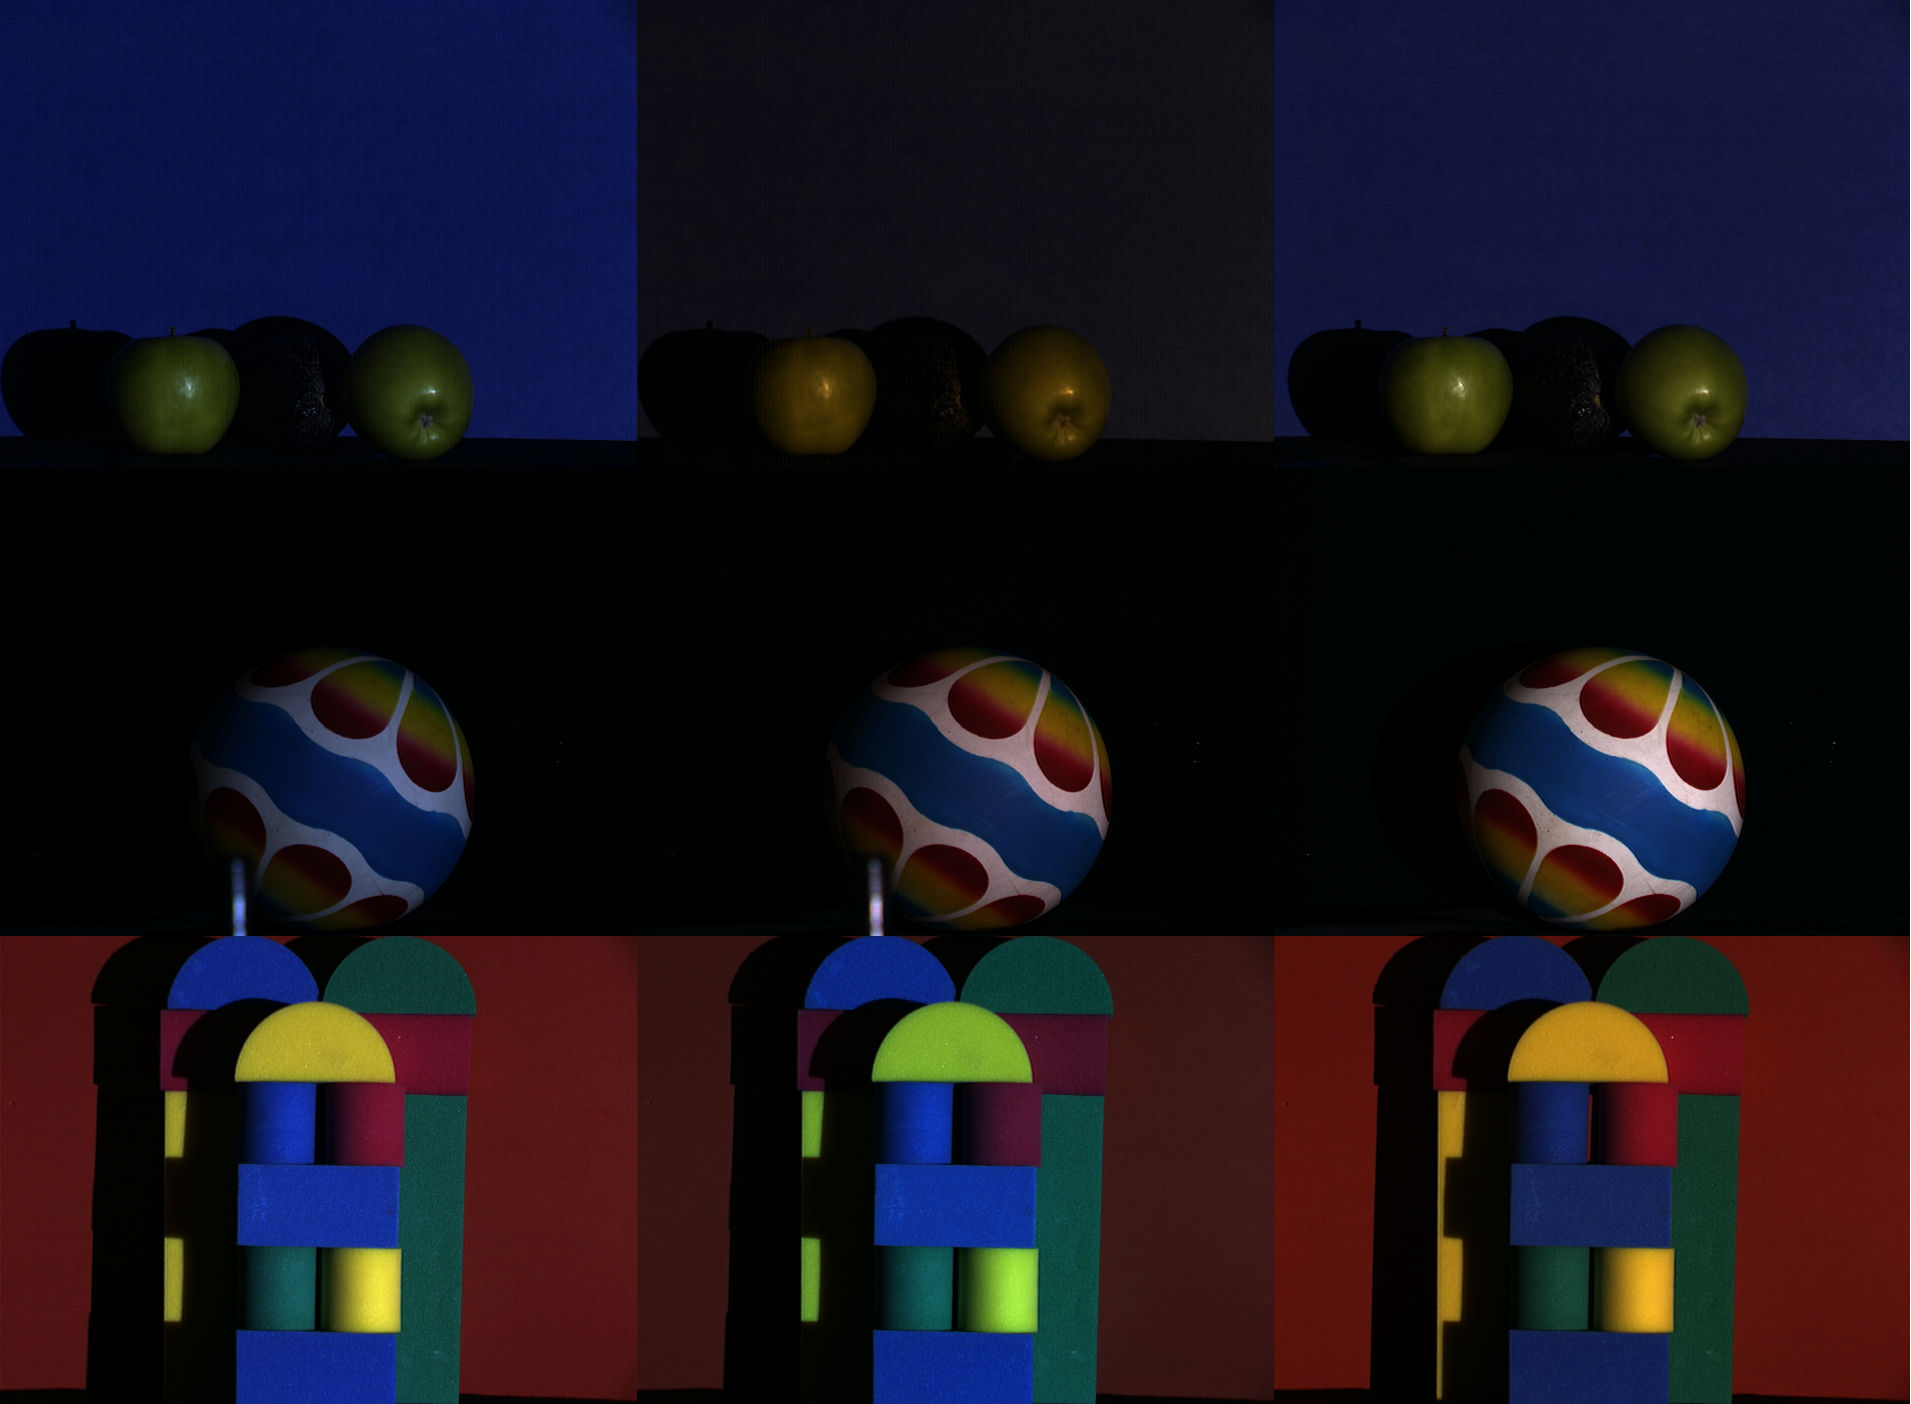
\includegraphics[width=120mm]{figs/results-grayworld-3x3.png}
	\caption{Left: The three scenes (apples, ball, blocks) lit by the blue light. This is the source. 
        Center: The scenes transformed from the blue light space to the white light space 
        using the gray world light value and the diagonal color model. 
        This is the prediction.
        Right: The scenes lit by the white light. This is the target.}
\end{figure}

The results using this method are pretty bad for the apples scene and the blocks 
scene. (However, it seems to do alright with the ball scene.) An understanding 
of how gray world works can tell us why the results are so bad and what's going 
on. Since gray world averages over all of the pixel values, larger color patches 
will tend to dominate the calculated value. In the first image, the background 
image is blue as lit by the white light. This brings the calculated light to be 
much bluer than it should be. (If the background were roughly gray, things would 
be alright.) To counteract this, the predicted result adds way too much yellow 
light (the opposite of blue). This makes the apples appear too red.

The blocks image has a similar problem because the background is red. The 
algorithm finds that the light color is actually red, due to this, and to 
counteract the red light, the prediction has way too much cyan added (the 
opposite of red).

The ball is unaffected by this, since its background is roughly gray/black. The 
results for the ball are actually quite good, with a better angular error than 
max RGB and a RMSE r,g value on par with max RGB.

\section{Minimizing Mean Squared Error using the Gradient}

The holy grail of many types of problems is the minimization of an error metric. 
Here, we consider the MSE metric:

$$
E = \frac{\sum^H_y \sum^W_x \sum_{c \in \{R, G, B\}} (\frac{L^T_c}{L^S_c} S_{x,y,c} - T_{x,y,c})^2}{3 H W}
$$

Where $H$ is the image height, $W$ is the image width, $L^T$ is the target 
light, $L^S$ is the source light, $S_{x,y,c}$ is the value of the source image at pixel 
$x, y$ for channel $c$, and $T_{x,y,c}$ is the value of the target image at pixel $x, y$ for 
channel $c$.

Our objective is to find the source light values that minimize this function:

$$
argmin_{L^S_R, L^S_G, L^S_B} (\frac{\sum^H_y \sum^W_x \sum_{c \in \{R, G, B\}} (\frac{L^T_c}{L^S_c} S_{x,y,c} - T_{x,y,c})^2}{3 H W})
$$

To do so, we compute the gradient of that equation with respect to the three 
source light channels, then set that gradient to the 0 vector, then solve. (Note 
that I think the non-homogeneous LSE method using the pseudoinverse would work 
as well, but I used the gradient method instead. I think the two answers are 
equivalent.) Each 
channel is symmetric and will have a very similar partial derivative, so let's 
just consider $\frac{\delta E}{\delta L^S_R}$:

\begin{align*}
\frac{\delta E}{\delta L^S_R} &\propto - \sum^H_y \sum^W_x (\frac{L^T_R}{L^S_R} S_{x,y,R} - T_{x,y,R}) (\frac{L^T_R}{(L^S_R)^2} S_{x,y,R}) \\
                              &\propto \sum^H_y \sum^W_x (\frac{L^T_R}{L^S_R} (S_{x,y,R})^2) - \sum^H_y \sum^W_x (T_{x,y,R} S_{x,y,R})
\end{align*}

Setting the gradient to 0, we have:

\begin{align*}
\sum^H_y \sum^W_x (T_{x,y,R} S_{x,y,R}) &= \sum^H_y \sum^W_x (\frac{L^T_R}{L^S_R} (S_{x,y,R})^2) \\
\sum^H_y \sum^W_x (T_{x,y,R} S_{x,y,R}) &= \frac{L^T_R}{L^S_R} \sum^H_y \sum^W_x (S_{x,y,R})^2 \\
L^S_R &= L^T_R \frac{\sum^H_y \sum^W_x (S_{x,y,R})^2}{\sum^H_y \sum^W_x (T_{x,y,R} S_{x,y,R})}
\end{align*}

Similar for the remaining two channels. This is the expression which we will 
solve for. At this point, it should be noted that, since all three channels are 
independent of each other, and each individual result in the sum is squared and 
thus is guaranteed to be positive, surely minimizing the error result for all three 
channels will also minimize the error result in just the r,g channels, so this 
\textit{should} also minimize the RMSE r,g metric. Computing this minimum gives 
us the following results:

The lights recovered using this method follow:

\begin{tabular}{r | r r r}
                 & Red & Green & Blue \\
    \hline                            \\
    Apples Light & 131 &   159 &  250 \\
      Ball Light & 133 &   163 &  250 \\
    Blocks Light & 126 &   157 &  250
\end{tabular}

and the quantitative results:

\begin{tabular}{r | r r}
                 & Angular Error & RMSE r,g Error \\
    \hline                                        \\
    Apples Light &        0.0025 &         0.0159 \\
      Ball Light &        0.0084 &         0.0631 \\
    Blocks Light &        0.0158 &         0.0230
\end{tabular}

And the qualitative results:

\begin{figure}[!ht]
	\centering
	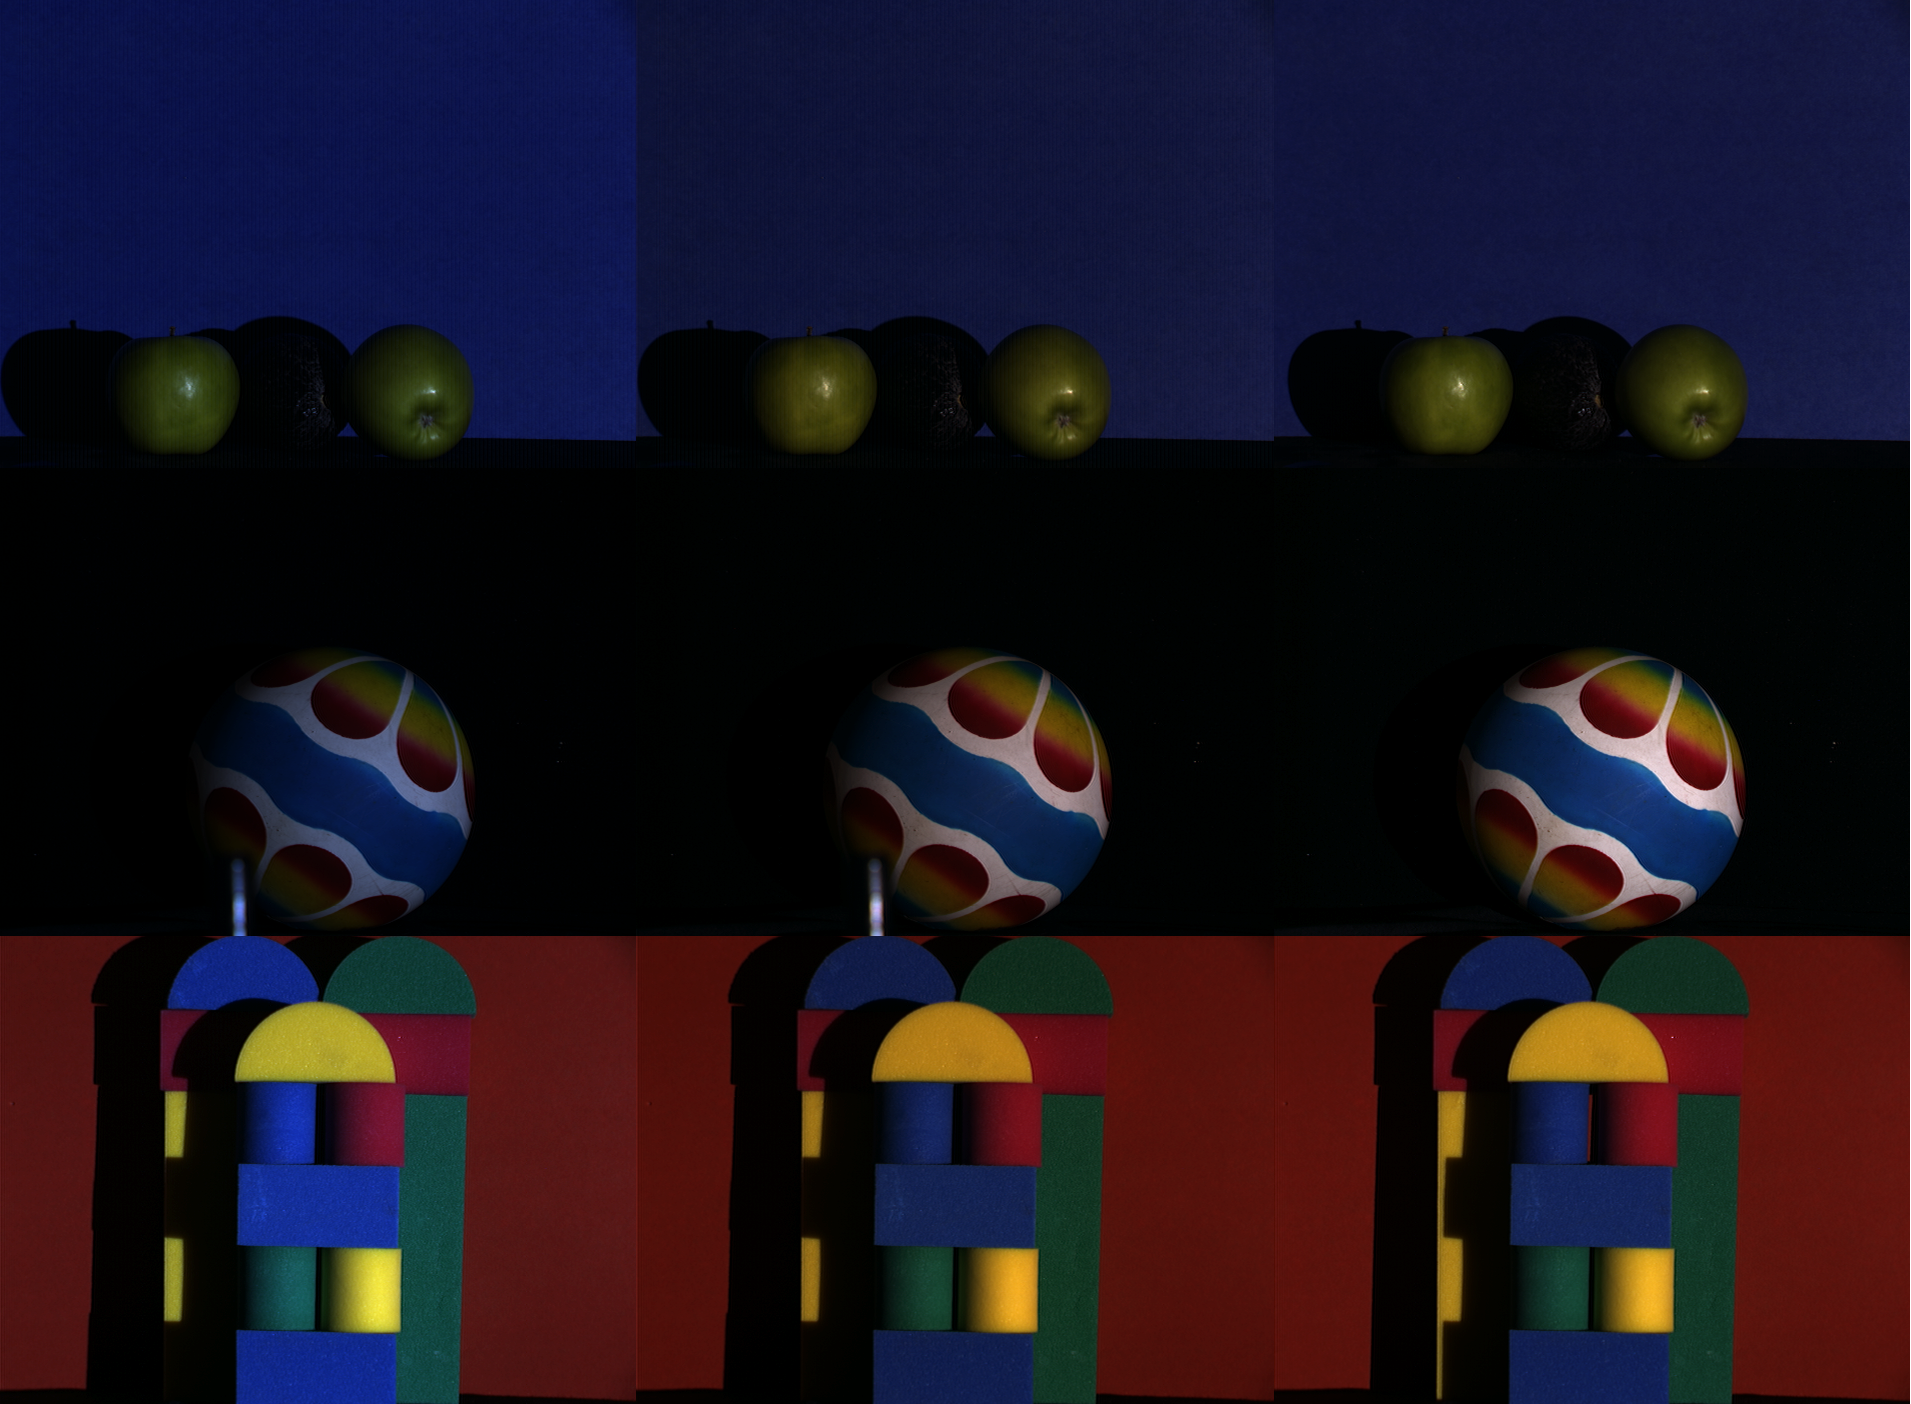
\includegraphics[width=120mm]{figs/results-msemin-3x3.png}
	\caption{Left: The three scenes (apples, ball, blocks) lit by the blue light. This is the source. 
        Center: The scenes transformed from the blue light space to the white light space 
        using the minimum MSE light value and the diagonal color model. 
        This is the prediction.
        Right: The scenes lit by the white light. This is the target.}
\end{figure}

The predictions are remarkably good. The ball result is a little worse than 
expected, due to the abberation to the bottom-left of the ball. Examining the 
light values show that the predicted lights are very close to each other for 
each scene. The error metrics are also very good.

\section{Off-the-shelf Optimization Method}

Matlab provides a function for finding minimum values for a given, arbitrary 
function. One such method is "simulannealbnd," which implements the simulated 
annealing strategy, and enforces a given bound on the final output vector. The 
simulated annealing strategy is good for finding a global minimum, as opposed to 
a local minimum. We can simply use the RMSE r,g function that we already have 
defined to do so. Comparing the results should give us some more evidence for 
whether minimizing the MSE actually minimizes the RMSE r,g as well.

The lights recovered using this method follow:

\begin{tabular}{r | r r r}
                 & Red & Green & Blue \\
    \hline                            \\
    Apples Light & 128 &   156 &  250 \\
      Ball Light & 146 &   172 &  250 \\
    Blocks Light & 135 &   159 &  250
\end{tabular}

and the quantitative results:

\begin{tabular}{r | r r}
                 & Angular Error & RMSE r,g Error \\
    \hline                                        \\
    Apples Light &        0.0130 &         0.0141 \\
      Ball Light &        0.0434 &         0.0606 \\
    Blocks Light &        0.0060 &         0.0148
\end{tabular}

The results are a bit unexpected and reveal that the minimum MSE measurement 
does not actually minimize the RMSE r,g values, since these are slightly better. 
I had originally thought that, since the three color channels are independent, 
the answer which minimizes the MSE would also minimize the RMSE r,g value. 
However, taking a closer look at the RMSE r,g metric reveals that the colors are 
\textit{not} actually independent in this metric:

\begin{align*}
r = \frac{R}{R + G + B} \\
g = \frac{G}{R + G + B} \\
b = \frac{B}{R + G + B}
\end{align*}

Since this metric essentially takes proportion, rather than raw value, into 
account, the channels are not independent, so the answer which minimizes the MSE 
will be different from the answer that minimizes the RMSE r,g.

\end{document}